%% Version 4.3.1, 19 May 2014
%
%%%%%%%%%%%%%%%%%%%%%%%%%%%%%%%%%%%%%%%%%%%%%%%%%%%%%%%%%%%%%%%%%%%%%%
% Template.tex --  LaTeX-based template for submissions to the 
% American Meteorological Society
%
% Template developed by Amy Hendrickson, 2013, TeXnology Inc., 
% amyh@texnology.com, http://www.texnology.com
% following earlier work by Brian Papa, American Meteorological Society
%
% Email questions to latex@ametsoc.org.
%
%%%%%%%%%%%%%%%%%%%%%%%%%%%%%%%%%%%%%%%%%%%%%%%%%%%%%%%%%%%%%%%%%%%%%
% PREAMBLE
%%%%%%%%%%%%%%%%%%%%%%%%%%%%%%%%%%%%%%%%%%%%%%%%%%%%%%%%%%%%%%%%%%%%%

%% Start with one of the following:
% DOUBLE-SPACED VERSION FOR SUBMISSION TO THE AMS
%\documentclass{ametsoc}

% TWO-COLUMN JOURNAL PAGE LAYOUT---FOR AUTHOR USE ONLY
\documentclass[twocol]{ametsoc}

%%%%%%%%%%%%%%%%%%%%%%%%%%%%%%%%
%%% To be entered only if twocol option is used

\journal{jcli}

%  Please choose a journal abbreviation to use above from the following list:
% 
%   jamc     (Journal of Applied Meteorology and Climatology)
%   jtech     (Journal of Atmospheric and Oceanic Technology)
%   jhm      (Journal of Hydrometeorology)
%   jpo     (Journal of Physical Oceanography)
%   jcli      (Journal of Climate)
%   mwr      (Monthly Weather Review)
%   wcas      (Weather, Climate, and Society)
%   waf       (Weather and Forecasting)
%   bams (Bulletin of the American Meteorological Society)
%   ei    (Earth Interactions)

%%%%%%%%%%%%%%%%%%%%%%%%%%%%%%%%
%Citations should be of the form ``author year''  not ``author, year''
\bibpunct{(}{)}{;}{a}{}{,}

%%%%%%%%%%%%%%%%%%%%%%%%%%%%%%%%

%%% To be entered by author:

%% May use \\ to break lines in title:

%\title{Atmospheric response to simulated historical sea ice loss}
\title{Isolating the impact of human-induced Arctic sea ice loss on the atmosphere}

%%% Enter authors' names, as you see in this example:
%%% Use \correspondingauthor{} and \thanks{Current Affiliation:...}
%%% immediately following the appropriate author.
%%%
%%% Note that the \correspondingauthor{} command is NECESSARY.
%%% The \thanks{} commands are OPTIONAL.

    %\authors{Author One\correspondingauthor{Author One, 
    % American Meteorological Society, 
    % 45 Beacon St., Boston, MA 02108.}
% and Author Two\thanks{Current affiliation: American Meteorological Society, 
    % 45 Beacon St., Boston, MA 02108.}}

\authors{Kelly E. McCusker\correspondingauthor{School of Earth and Ocean Sciences, University of Victoria, Victoria, BC, Canada.}}

%% Follow this form:
    % \affiliation{American Meteorological Society, 
    % Boston, Massachusetts.}

\affiliation{University of Victoria,
                      Victoria, British Columbia}

%% Follow this form:
    %\email{latex@ametsoc.org}

\email{kemccusk@uvic.ca}

%% If appropriate, add additional authors, different affiliations:
    %\extraauthor{Extra Author}
    %\extraaffil{Affiliation, City, State/Province, Country}

\extraauthor{John C. Fyfe}
%\extraaffil{}

%% May repeat for a additional authors/affiliations:

\extraauthor{Michael Sigmond}
\extraaffil{University of Victoria,
                      Victoria, British Columbia}



%%%%%%%%%%%%%%%%%%%%%%%%%%%%%%%%%%%%%%%%%%%%%%%%%%%%%%%%%%%%%%%%%%%%%
% ABSTRACT
%
% Enter your Abstract here

%\abstract{Changes in Arctic sea ice play an important role in modulating surface fluxes of heat and moisture, and therefore local near-surface temperatures and precipitation. Whether or not historical sea-ice retreat has had a marked influence on weather patterns, particularly outside the local region, remains an open and important question. Here the effect historical sea-ice loss has on the atmosphere is isolated by prescribing observed sea-ice concentrations and local sea surface temperatures in an atmosphere model. A suite of 120-year simulations is carried out to temper natural variability. We find that observed boundary conditions produce a lowering of Arctic sea level pressure in Autumn that is robust and consistent with other studies, but no clear signal in patterns of variability emerge. Furthermore, the response to observed sea-ice changes is compared to a suite of simulations in which boundary conditions are obtained from an ensemble of historical simulations from a coupled global climate model. We find that whereas near-surface temperature responds in accordance with the amount of sea ice loss --- more loss yields larger warming --- sea-level pressure and geopotential heights remain slave to natural variability. Individual ensemble members have regions and seasons of statistically significant circulation changes in response to sea-ice loss, however those regions and seasons are not robust across ensemble members. Thus, it is likely that 1. historical sea-ice loss played a minimal role in setting circulation trends and 2. any detectable effect sea-ice loss had is due to @@ Thus, caution must be taken when interpreting even long time-slice simulations  @@. Notably, the observed forcing produces a response that is outside the bounds of the } % Harder to tease out is how changes in sea ice influence local and remote circulation. % natural variability for determining both the sea-ice forcing pattern and the response to sea-ice loss by prescribing an ensemble of boundary conditions obtained from a coupled model's ensemble of historical simulations. %...@@. The importance of the pattern of sea-ice loss is further examined by prescribing a suite of boundary conditions obtained from a coupled model's ensemble of historical simulations. 


%Isolating the Impact of human-induced Arctic Sea Ice Loss on the Atmosphere

\abstract{Changes in Arctic sea ice play an important role in modulating surface fluxes of heat and moisture, and therefore local near-surface temperatures and precipitation. Whether or not historical sea-ice retreat has had a marked influence on remote climatic changes remains an open and important question. Here the effects of historical sea-ice loss on the atmosphere are isolated by prescribing Arctic sea ice loss from two different observational datasets to an atmosphere-only model. In addition, we prescribe to the atmosphere-only model sea ice loss patterns simulated by an ensemble of historical simulations with the corresponding coupled model. These simulations allow for the separation of the climate effects of forced (human-induced) sea ice loss and the climate effects of (random) sea ice changes induced by internal variability. We find that all scenarios exhibit a robust, shallow Arctic warming, a tendency for lower Arctic sea level pressure, and higher geopotential heights aloft in Autumn and Winter. However, the pattern and magnitude of circulation change outside the Arctic and at upper levels varies widely across simulations. We suggest that internal variability in the sea ice anomaly pattern itself is an important driver in determining surface temperature changes and aspects of circulation changes to observed Arctic sea ice loss.
} % Slightly modified AGU Abstract. We suggest that internal variability in the sea ice anomaly pattern itself is an important driver in determining midlatitude changes to observed Arctic sea ice loss. 


\begin{document}

%% Necessary!
\maketitle


%%%%%%%%%%%%%%%%%%%%%%%%%%%%%%%%%%%%%%%%%%%%%%%%%%%%%%%%%%%%%%%%%%%%%
% MAIN BODY OF PAPER
%%%%%%%%%%%%%%%%%%%%%%%%%%%%%%%%%%%%%%%%%%%%%%%%%%%%%%%%%%%%%%%%%%%%%
%

%% In all cases, if there is only one entry of this type within
%% the higher level heading, use the star form: 
%%
% \section{Section title}
% \subsection*{subsection}
% text...
% \section{Section title}

%vs

% \section{Section title}
% \subsection{subsection one}
% text...
% \subsection{subsection two}
% \section{Section title}

%%%
% \section{First primary heading}

% \subsection{First secondary heading}

% \subsubsection{First tertiary heading}

% \paragraph{First quaternary heading}

\section{OUTLINE}

\subsection{Motivation}

Obvious motivations: sea ice is diminishing, sea ice loss is important for various reasons, lots of chatter about polar amplification caused by sea ice loss affecting midlatitude weather, etc.\\
This is the first attempt to examine the isolated impact of sea ice loss in the Canadian AGCM. Previous works have used models from two model lineages: NCAR Community GCM, and Hadley GCMs (with the exception of one study using ECHAM). CanESM sea ice trend is very good, but mean state biased very low (in Sep).\\
Internal variability plays an almost equal role to external forcing in determining the sea ice pattern (Kay et al, Stroeve et al, Wettstein and Deser?), therefore it is an important contributor to any linkages drawn between observed sea ice loss and remote circulation changes. As such, we attempt to separate the effect of human-induced sea ice loss on the local and remote atmosphere from the effect that the internal variability in the sea ice pattern has on the atmosphere.\\
We have effectively created a large ensemble of simulations in which the atmosphere reacts to various realizations of prescribed sea ice. Two ensembles of 5 perturbed and 5 control sea ice simulations each, plus 2 pair of observational sea ice forcings, and 3 pair of additional sensitivity simulations, all 120 years in length. In total, we have 30*120 years of simulations = 2,400 years.\\
We are able to draw some heretofore previously un-proven conclusions about the effect historical sea ice loss has on the atmosphere.

\subsection{Mean obs runs (HAD and NSIDC)}
Focus on temperature response as it is converged after 120 years.\\
Describe circulation responses. Relate to previous results where applicable.\\

SUMMARY:\\
Autumn, polar SAT response in HAD is slightly warmer than NSIDC, and extends further outside the Arctic in some locations. Given that HAD has slightly less ice loss than NSIDC in SON, this must be explained by internal variabilty in the response (Figure \ref{fig:fig3} and Figure \ref{fig:f1b}). SLP is lowered over the polar cap in both HAD and NSIDC, with the deepest lows in NSIDC over much of the Arctic ocean and northern Canada / Hudson's Bay. Only NSIDC has a statistically significant lowering of SLP over the polar cap. Both simulations also have a strengthening of the Siberian high (?).  \\

HAD displays a significant region of high geopotential heights extending over Barents-Kara, Laptev, East Siberian, and Chukchi Seas, and extending south over north and east Siberia in SON, whereas NSIDC has a much smaller region of high heights over north-central Siberia but insignificant low heights over the polar cap (Figure \ref{fig:fig3c}). Accordingly, the $>$65N average (NAM index) is significant and positive (negative NAM) in HAD with no significant change in NSIDC. Is this difference due to the sea ice forcing pattern or internal variability in the response? Ice loss patterns look similar in SON (by eye), but NSIDC has more polar cap ice loss in SON, especially in the B-K-S region, yet smaller Z500 response -- this implies it is internal variability in the response. This is consistent with what we find later when examining the ANT and TOT ensembles.\\

The winter and spring SAT response in HAD is significantly affected by the bias in sea ice loss (not enough loss) in the HadISST dataset in winter and spring. This is particularly apparent in DJF when there is significant cooling over the polar cap in HAD but not NSIDC (Figure \ref{fig:fig3} and Figure \ref{fig:f1b}). The result is that HAD does not have a statistically significant lowering of SLP over the polar cap, while NSIDC does, primarily due to SLP over the Greenland, Barents, and Kara seas. Additionally, while the pattern of SLP response is similar between HAD and NSIDC, the magnitudes in HAD are smaller, with neither exhibiting large regions of statistically significant response (Figure \ref{fig:fig3b}). Z500 patterns in DJF are similar between HAD and NSIDC, but have different statistically significant regions (Figure \ref{fig:fig3c}). The implication is that the DJF sea ice loss bias does not significantly alter the circulation response. \\

DJF $>$65N Z500 anomalies are insignificant in both observational simulations, with no consistent and significant regional changes between the two simulations. However, both show high heights over the North Atlantic, North America, and north-central Russia (Barents-Kara Seas area), and low heights over the North Pacific. The statistically significant high height found over the Barents-Kara Seas in HAD is similar to that found to cause cold-Eurasian winters (e.g. Mori et al 2014), although we do not find statistically significant cooling there in the DJF time-mean (refer to Figure \ref{fig:fig3}). February does however have a region of significant cooling in central Eurasia in HAD. Both January and February exhibit significant cooling in NSIDC although the region extends somewhat further south near Kazakhstan and northern China/Mongolia.\\

Associated with the Z500 anomalies, the only significant upper-level zonal wind (300hPa) anomalies appear in HAD in SON where there is a significant weakening of the westerlies over eastern Russia (poleward of the pacific jet; Figure \ref{fig:fig3d}). Accordingly, zonal mean zonal wind does not show a significant or robust zonal mean response with altitude.\\

Comparison with previous studies with HadISST:\\
SAT response is similar to Peings and Magnusdottir 2014 (PM14) DJF and Screen, Deser et al. 2013 (SD13) SON and DJF. \\
Although difficult to discern from the figures, HAD Z500 in DJF resembles the results of PM14 in that they both have a small, statistically significant high over the BKS, but our study lacks the significant region of high height over the Atlantic from about 30-45N. Additionally, Screen, Simmonds et al 2013 (SS13) find Z500 highs over the N. Atlantic/Greenland in early winter that are not significant, similar to our results, but only show a high near BKS in CAM3 (not UM7.3) in S-O. Note that these studies are not directly comparable as they have different periods of sea ice forcing and SS13 is transient.\\
We confirm with larger ensembles that increased geopotential heights over the North Atlantic / GIN seas / Greenland are a robust response to historical sea ice loss in DJF (as is a high over northeastern Russia and Sea of Okhotsk).\\ %@@ ? Also similar to PM14, we find a negative NAM response that does not project onto surface variables such as SLP and SAT.

We will discover in the following sections that while the atmosphere does exhibit statistically significant circulation responses to sea ice loss that can be explained in a physically consistent way, an important driver of the response is still atmospheric internal variability, and secondarily internal variability in the sea ice pattern.\\

FIGURES:\\
-Latitude by month SAT anomaly plus SIC anomaly contours. Potentially add bar graph of polar average net flux to same fig. Panels for HAD, NSIDC, $\overline{TOT}$ (?), $\overline{ANT}$\\
-Seasonal cycle polar average quantities. Panels for SIA, NET flux, SAT, SLP, Z500 (and PREC?). This figure will show TOT mean and range, ANT mean, HAD, NSIDC all on one figure.\\
-NH anomaly maps. Panels for SAT, SLP, Z500, U300(?) response for HAD, NSIDC, $\overline{TOT}$, $\overline{ANT}$ for SON and DJF.\\
-NH zonal mean with height. Panels for temp, zonal wind, geopotential height in HAD, NSIDC, $\overline{TOT}$, $\overline{ANT}$ for SON and DJF \\

\subsection{Internal variability in the BCs}

Part of the historical, observed sea ice loss is due to internal variability rather than external (aka human -induced or anthropogenic) forcing (about 40\% cite Kay et al, Stroeve et al). \\
In order to quantify the contribution of internal var in the sea ice pattern to the response to sea ice loss, we run 5 pair of 120-year simulations with individual boundary conditions taken from the historical ensemble members in the corresponding GCM, CanESM2. Each ensemble member represents the response to a 'total' (TOT) boundary condition that includes anthropogenic sea ice loss plus internal variability. \\
To isolate the response to human-induced sea ice loss, we then execute 5 additional pair of 120-year simulations in which the boundary condition for all ensemble members is identically the average of the 5 TOT ensemble member boundary conditions. We assume this average boundary condition is the human-induced boundary condition. Therefore, this ensemle represents the response to anthropogenic-only sea ice loss (ANT).\\
A comparison of $\overline{TOT}$ to $\overline{ANT}$ (where the overbar indicates the average of the respective ensemble members) allows us to examine the importance of internal variability in the sea ice boundary condition to the response to that boundary condition. If the response in $\overline{TOT}$ is about equal to the response in $\overline{ANT}$, then i. the response to individual TOT forcings is additive and ii. the response to various representations of sea ice loss is primarily due to human-induced sea ice loss, and not internal variability in the ice pattern. Alternatively, differences between $\overline{TOT}$ and $\overline{ANT}$ imply that internal variability in the sea ice forcing pattern is important to the response.\\

% SON range in ENS: 0.45458     0.45/1.17 = 0.38 = 38% of mean
% SON range in ENSE: 0.09009   0.09/1.12 = 0.08 = 8% of mean
% SON ENS 1.16884,  ENSCI:      (1.14461,   1.19307)
% SON ENSE 1.12262,  ENSECI: (1.09886,   1.14637) % Technically SON polar temp is statistically separated at the 4th decimal place.....

% DJF range in ENS: 0.44108     0.44/1.06 = 0.42 = 42% of mean
% DJF range in ENSE: 0.35847   0.36/1.09 = 0.33 = 33% of mean
% DJF ENS 1.06015,  ENSCI:       (1.00224,   1.11807)
% DJF ENSE 1.08724,   ENSECI: (1.02887,   1.14562) % Not statistically separated

\subsubsection{Compare $\overline{TOT}$ with $\overline{ANT}$}

$\overline{TOT}$ generally has more defined, larger regions of statistically significant response in circulation variables such as SLP, Z500, and U300 in SON and DJF than $\overline{ANT}$ (the one exception is SLP in SON). This is contrary to what one might expect given that ANT is comprised of 600 years of response to the same boundary condition, whereas TOT is comprised of 600 years of response to 5 different boundary conditions. The implication is that internal variability in the sea ice pattern, while not drastically altering the circulation response, does amplify the response.\\

We surmise that the reason for this is the uniformity of boundary condition in $\overline{ANT}$. The suggestion is that smaller, more defined regions of sea ice anomalies are more effective at forcing the atmosphere into a particular state through generation of Rossby waves (causing blocking patterns), whereas broader, more uniform regions of sea ice anomalies generate Rossby waves that may destructively interfere with each other, allowing the polar circulation to wander more and not settle --- essentially remaining unforced. @@\\

The SAT response in the mean of both ensembles is nearly identical in SON and DJF, both in magnitude (see seasonal cycle or regional mean figure of seasonal polar cap temp anomalies), and pattern (see pattern correlation of 0.99 and 0.98 for SON and DJF, respectively). Describe.\\
$\overline{TOT}$ and $\overline{ANT}$ polar cap ($>$60N) ensemble mean SAT anomalies are similar (1.17, 1.12$^\circ$C in SON and 1.06, 1.09$^\circ$C in DJF), and not statistically different from each other (technically, the SON average SAT anomalies are juuuust separated as the upper confidence limit on $\overline{ANT}$ is 0.0002 lower than the lower confidence limit on $\overline{TOT}$).\\ 

Describe lowering of SLP over polar cap in SON, broader in $\overline{ANT}$. No significant SLP response over the polar cap in DJF, but both ensemble means share a significant lowering over Hudon's Bay, Baffin Bay, Davis Strait, Labrador Sea. Pattern correlations are relatively high at 0.75 and 0.67 for SON and DJF, respectively.\\
There is a greater area of significant SLP response in $\overline{TOT}$ in DJF which may indicate amplification of the response to anthropogenic ice loss by internal variability in the ice pattern as described above.\\

In SON, Z500 is anomalously high over the polar cap, with a broader significant region and a greater polar average anomaly magnitude in $\overline{TOT}$ than in $\overline{ANT}$. \\

Z500 in DJF (and secondarily SON) is the most robust circulation response. Both ensemble means exhibit polar average high Z500 (a negative NAM index) that are statistically significant, with strong high lobes over the North Atlantic/GIN Seas, and Northeast Siberia including the Sea of Okhotsk. The pattern correlation between $\overline{TOT}$ and $\overline{ANT}$ is 0.78 (or 62\% common variation). The resulting zonal wind (U300) anomalies display weakened Pacific and Atlantic jets on the poleward side, and strengthening on the eqatorward side, indicating a southward shift of the storm tracks. $\overline{TOT}$ has a greater amplitude of response and larger areas of significance, including upper level zonal wind (U300; Figure \ref{fig:fig3d}).\\ 

\subsubsection{Compare TOT and ANT ensembles}
The going assumption in recent literature has been that 60-100 years of simulation is adequate to determine the forced local, circulation response to sea ice loss. Here we increase the sample size to 120 years per simulation pair. If 120 years is sufficient to result in a robust pattern of response, then we would expect that each ensemble member in ANT --- which all have the same boundary condition (forcing) --- will have essentially the same time-average response. Then, any deviations between TOT ensemble members is due to internal variability in the sea ice pattern (forcing).\\

ANT ensemble members all have roughly equivalent polar cap ($>$60N) SAT anomalies in SON, indicating that 120 years is sufficient to filter out most internal variability in the SAT response to sea ice loss. However, because each ensemble member in ANT only varies because of internal variability in the response, we can estimate the portion of the SON SAT response due to internal variability in the response by comparing the range of polar cap SAT anomalies to the mean anomaly; if internal variability was not a factor, all ensemble members would have the same polar cap anomaly. The range of SON polar cap SAT anomalies in ANT is 0.09$^\circ$C which is 8\% of the average anomaly and is due to internal variability in the response. In contrast, the range in polar cap SAT anomalies in TOT is 0.45$^\circ$C (38\%).\\

Removing the estimate of internal variability in the response (8\%), we find that 30\% of the magnitude of SAT response in TOT is due to internal variability in the sea ice anomaly pattern. Because TOT ensemble members exhibit this large range in polar cap SAT anomalies that is 30\% of the mean (after removing the contribution from internal variability in the response), we can conclude that internal variability in the sea ice forcing pattern is an important driver of the magnitude of the SAT response in SON. This contribution of 30\% is also comparable to previous estimates of the contribution of internal variability to observed sea ice loss of around 40\%. \\

Moving on from polar cap averages, we can estimate internal variabilty in the pattern itself by calculating pattern correlations between ensemble members. If we correlate the SAT response pattern of each TOT ensemble member with each other to quantify how similar each response pattern is to another equally probable sea ice evolution, we see that the average 'percent common variation', or average of the squared-correlation coefficients, gives 70\% for the TOT ensemble compared with 90\% for the ANT ensemble. This indicates that i. about 10\% of the SAT response pattern in ANT is internal variability in the response (100-90\%, since the sea ice forcing pattern is identical for all members and 120 years per member gives a robust response), and ii. about 20\% of the SAT response in TOT is internal variability in forcing pattern + internal variability in response (90\%-70\%), yielding a residual of 10\% contribution from internal variability in the sea ice pattern. This implies that internal variability in the sea ice pattern itself is of equivalent importance to internal variability in the response to sea ice loss for determining the pattern of SAT response. \\

In summary then, for determing the SON SAT response pattern, internal variability in the sea ice anomaly pattern is as important as internal variability in the response to that ice anomaly (10\% vs 10\%). Similarly, average polar cap SAT anomaly magnitudes are influenced by internal variability in the response (8\%), internal variability in the sea ice forcing pattern (30\%), and anthropogenic sea ice loss (the residual of 62\%). \\ %@@quantify or at least pick out where/why this would be important weather-wise --- mainly local effect ?

The DJF SAT response within the ANT ensemble begins to display an influence from internal variability in the response as the range of polar average SAT is 0.36$^\circ$C, which is 33\% of the mean anomaly, compared with a range of 0.44$^\circ$C (42\%) within the TOT ensemble. Thus, the contribution to the magnitude of SAT response from internal variability in the sea ice anomaly in DJF is 9\% compared with 33\% due to interval variability in the response (58\% due to anthropogenic sea ice forcing). Taking pattern correlations between ensemble members within each ensemble, we find the average percent common variation is 80\% in ANT versus 45\% in TOT. Thus, 20\% of the DJF SAT response pattern can be attributed to internal variability in the response (100-80\%), leaving 25\% of the response pattern in the TOT ensemble due to internal variability in the sea ice forcing pattern.

\subsection{Internal variability in the response}

Within ANT, which always has the same ice boundary conditions, we find periods in time of Eurasian and North American cooling, as well as cooling in the time mean for some ensemble members. However, the time-mean response of the ensemble average ($\overline{ANT}$) is primarily warming in these regions (especially N. America), indicating that i. 120 years is not sufficient to converge on midlatitude regional temperatures in SON or DJF (or there is no signal, period) and ii. the response to \textit{anthropogenic} sea ice loss (in this AGCM) is slight warming in Eurasia and North America. \\
In fact, internal variability in the sea ice pattern in $\overline{TOT}$ tends to magnify the warming in Eurasia in DJF as compared to $\overline{ANT}$ such that the mean anomaly is statistically significant and positive.\\
The implication is that observational cooling that has been linked to sea ice loss is due to internal variability in the ice loss pattern, or more likely, internal variability in the response. \\

In a simulation with RCP8.5 2032-2042 sea ice loss, we find an even smaller chance of Eurasian cooling (although there still exists some years with cooler Eurasian SAT). Eurasian cooling will likely be a transient phenomenon and will not be the norm as global warming progresses due to well-mixed greenhouse gases. % (@@what does ENS look like...). 

\subsection{Conclusions}

i. 120 years is more than enough time to obtain a robust polar SAT response to ice loss in SON. (essentially no spread in the ANT ensemble regional mean. High pattern corrs). \\
ii. [NEW] Internal variability in the sea ice pattern is an important driver in the SON temperature response (30\%; compare with 62\% due to anthropogenic sea ice loss).\\% The range of TOT ensemble members is about 40\% of the mean anomaly (0.5/1.2C by eye). (pattern correlation useful here? TOT avg 70\%, ANT avg 90\% and less than 1/2 the spread)\\
iii. [NEW] Alternatively, internal variability in the sea ice pattern remains an influential component for the DJF temperature response (9\%; compare with 58\% due to anthropogenic sea ice loss), while internal variability in the response becomes more important (33\%). Comparing the range of pattern corrs between the individual ANT ensemble members and the individual TOT ensemble members, the response patterns are more similar in ANT (avg 80\%) than in TOT (avg 45\%, double the spread) \\
iv. [NEW] Internal variability in the sea ice pattern amplifies the SON temperature response in NSIDC and HAD (smaller SIC anomalies, larger SAT anomalies). Surface wind anomalies support this, showing southerly flow (warm air advection) into the Arctic.\\
v. [NEW] positive Z500 anomaly (negative NAM index) response is robust in both SON and DJF for the historical time period (not previously shown).\\
vi. In CanAM4, even 120 years was not enough to settle on a converged circulation response even locally in some cases. Evidence for this is that the spread in SLP and Z500 especially in DJF is wider in ANT than in TOT, meaning with the same boundary conditions the ensemble members in ANT had different mean circulation anomalies after 120 years.\\
vii. [NEW but needs to be worked out more -- need evidence.] One explanation for wildly variable circulation responses within the ANT ensemble in SON and DJF could be the relative uniformity of the anthropogenic sea ice boundary condition. This may cause the polar vortex to weaken and wobble more and not settle on a pattern (this is not borne out in inter-annual standard deviation within ANT and TOT but it's not the correct timescale). In contrast, more regional sea ice forcing (Barents-Kara Seas, Sea of Okhotsk tend to cause rossby wave responses) may force a particular circulation pattern (blocking), keeping the spread tighter between ensemble members, and resulting in more significant responses in individual ensemble members and ultimately the ensemble mean. Although perhaps not entirely meaningful because of lack of regional statistical significance, this idea is consistent with the slightly higher average intra-ensemble pattern correlation in TOT compared with intra-ensemble pattern correlation in ANT in SON/DJF SLP and Z500. In this way, internal variability in the sea ice pattern acts to amplify the response to anthropogenic sea ice loss, which is consistent with the fact that there are generally larger areas of significance in the TOT ensemble mean than the ANT ensemble mean (except SLP in SON). This phenomenon (ANT spread considerably wider than TOT) mainly occurs in Oct, Nov, and Dec. for SLP and Z500. \\



\begin{table*}[t]
\caption{Model simulation details. Diff name is used when describing the results as anomalies; e.g. HAD means Hadpt - Hadctl. The sensitivity simulations are listed at the bottom of the table and their corresponding control simulation is CANctl1. All simulations have a constant annually-repeating set of boundary conditions and are run for 121 years with the first year disregarded for analysis.}\label{simstbl}
\begin{center}
\begin{tabular}{llcccccc}
\hline\hline
Diff Name & Sim & SIC & SIT & SST & BC Source & Notes\\
\hline
HAD &  HADctl   & 1979-89 & 1979-89 & 1979-89 & HadISST1.1 \\
         & HADpt &   2002-11 & 1979-89* & 2002-11 & HadISST1.1 & *SIT set to 0 where SIC 0 \\
            &                 &               &                &                &                     &     and @@\\
 NSIDC & NSIDCctl  &1979-89 & 1979-89 & 1979-89 & NSIDC \\
             & NSIDCpt &   2002-11 & 1979-89* & 2002-11 & NSIDC & *SIT set to 0 where SIC 0 \\
               &              &                &                 &               &              &   and @@\\
 TOT[1-5] & CANctlBC[1-5] & 1979-89 & 1979-89 & 1979-89  & CanESM2 historical ensemble members 1-5  & \\
                & CANptBC[1-5] &   2002-12 & 2002-12 & 2002-12 &  CanESM2 historical ensemble members 1-5  & \\
 \\
 ANT[1-5] &  CANctl[1-5] &    1979-89 & 1979-89 & 1979-89 & CanESM2 historical ensemble average & 1-5 have varied initial conditions \\
                   & CANpt[1-5] & 2002-12 & 2002-12 & 2002-12 &  CanESM2 historical ensemble average &  1-5 have varied initial conditions \\
  \hline
 \hline
 ANT1nosit   & CANpt1nosit &     2002-12 & 1979-89* & 2002-12 &  CanESM2 historical ensemble, & *SIT set to 0 where SIC 0. \\
                       &                       &                 &                  &              &       average, member 1             & \\
ANT1nosst  &  CANpt1nosst &      2002-12 & 2002-12 & 1979-89 &  CanESM2 historical ensemble  & \\
                        &                       &                 &                  &              &       average, member 1             & \\
TOT4nosit   &  CANptBC4nosit  &    2002-12 & 1979-89* & 2002-12 &  CanESM2 historical ensemble member 4 & *SIT set to 0 where SIC 0. \\
\hline
\end{tabular}
\end{center}
\end{table*}


\begin{figure}[t]
  \noindent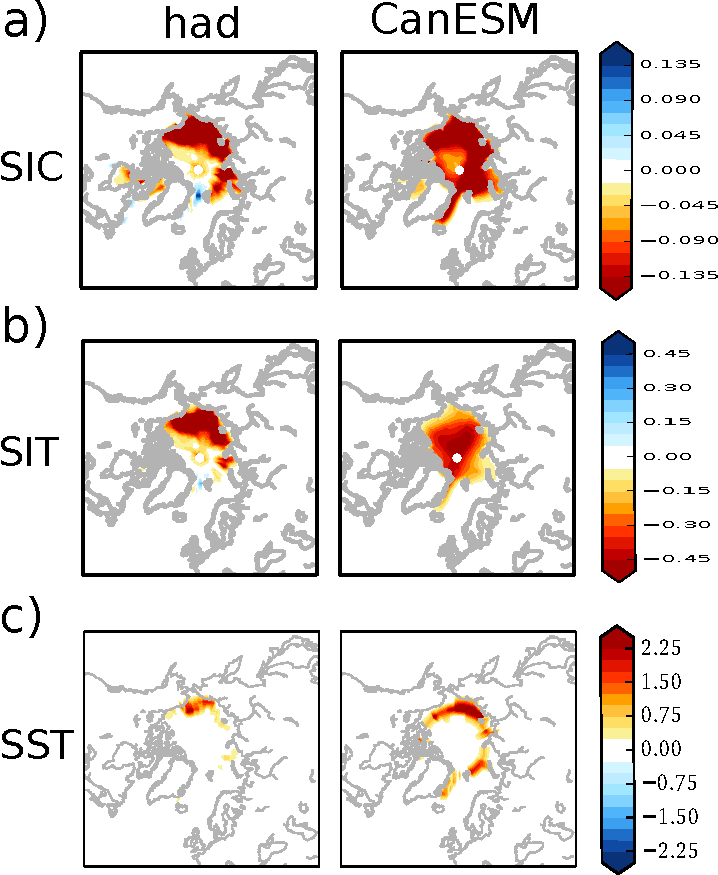
\includegraphics[width=19pc,angle=0]{oneseasBCsnonsidc.pdf}\\
  \caption{a) The difference in mean sea ice concentration (\%) prescribed as boundary conditions in HADctl (1979-89) and HADpt (2002-2011; left column) in Autumn (SON). The right column is as the left column but shows the difference between canPT and canCTL, respectively. b) and c) are as a) but show SIT and SST, respectively.
}\label{fig:fig1}
\end{figure}


\begin{figure}[t]
  \noindent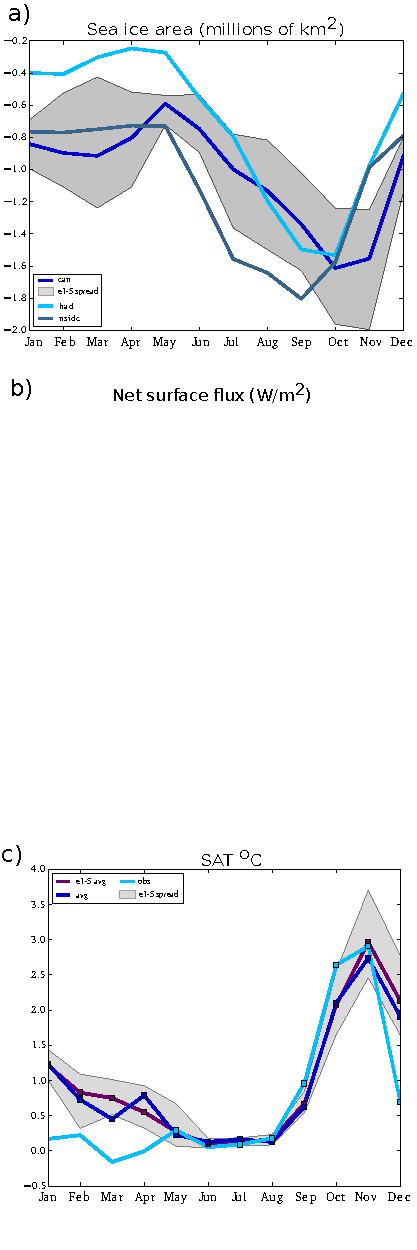
\includegraphics[width=15pc,angle=0]{seacycles.pdf}\\
  \caption{(old fig-- accidentally plotting North of 40N instead of 60N@@). Seasonal cycle of a.) Arctic sea ice area anomaly (10$^6$ km$^2$) for HAD (light blue), NSIDC (gray blue), CAN (dark blue), and ENS (magenta; exactly the same as CAN for sea ice area, by design). Gray shading indicates the range of sea ice area anomalies in individual ensemble members. b.) is as a) but for net surface flux anomaly averaged north of 40$^\circ$N where sea ice concentration $>$ 10\%, c.) is as a) but for surface air temperature anomaly averaged north of 70$^\circ$N, and d.) is as a) but for sea level pressure averaged north of 70$^\circ$N. Squares in b), c), and d) indicate a statistically significant anomaly at the 95\% level using a two-sided student's T test.
}\label{fig:fig2}
\end{figure}

\begin{figure*}[t]
  \noindent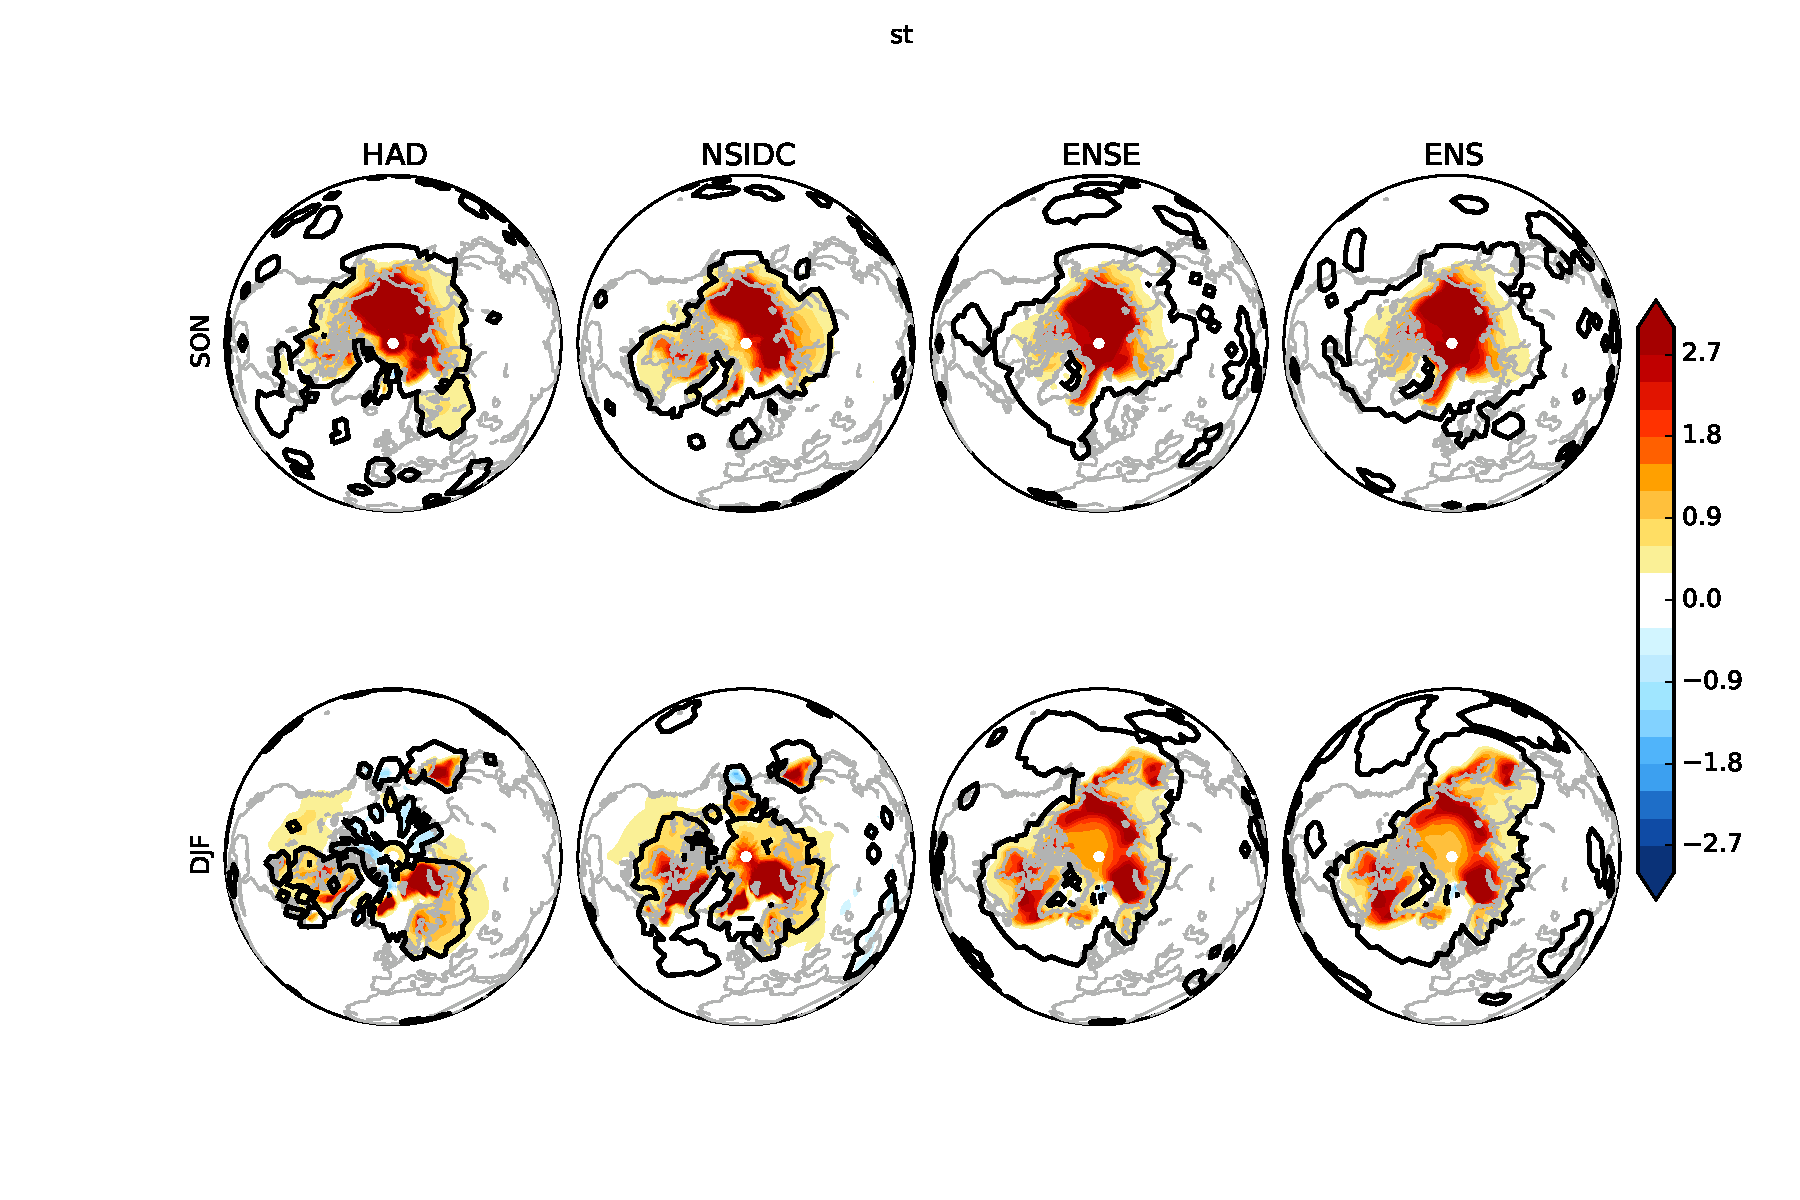
\includegraphics[width=35pc,angle=0]{stdiffsigcont_enssubplot_forpap3_seas_nh2.pdf}\\ %SATmaps.pdf}\\
  \caption{SAT maps
}\label{fig:fig3}
\end{figure*}

\begin{figure*}[t]
  \noindent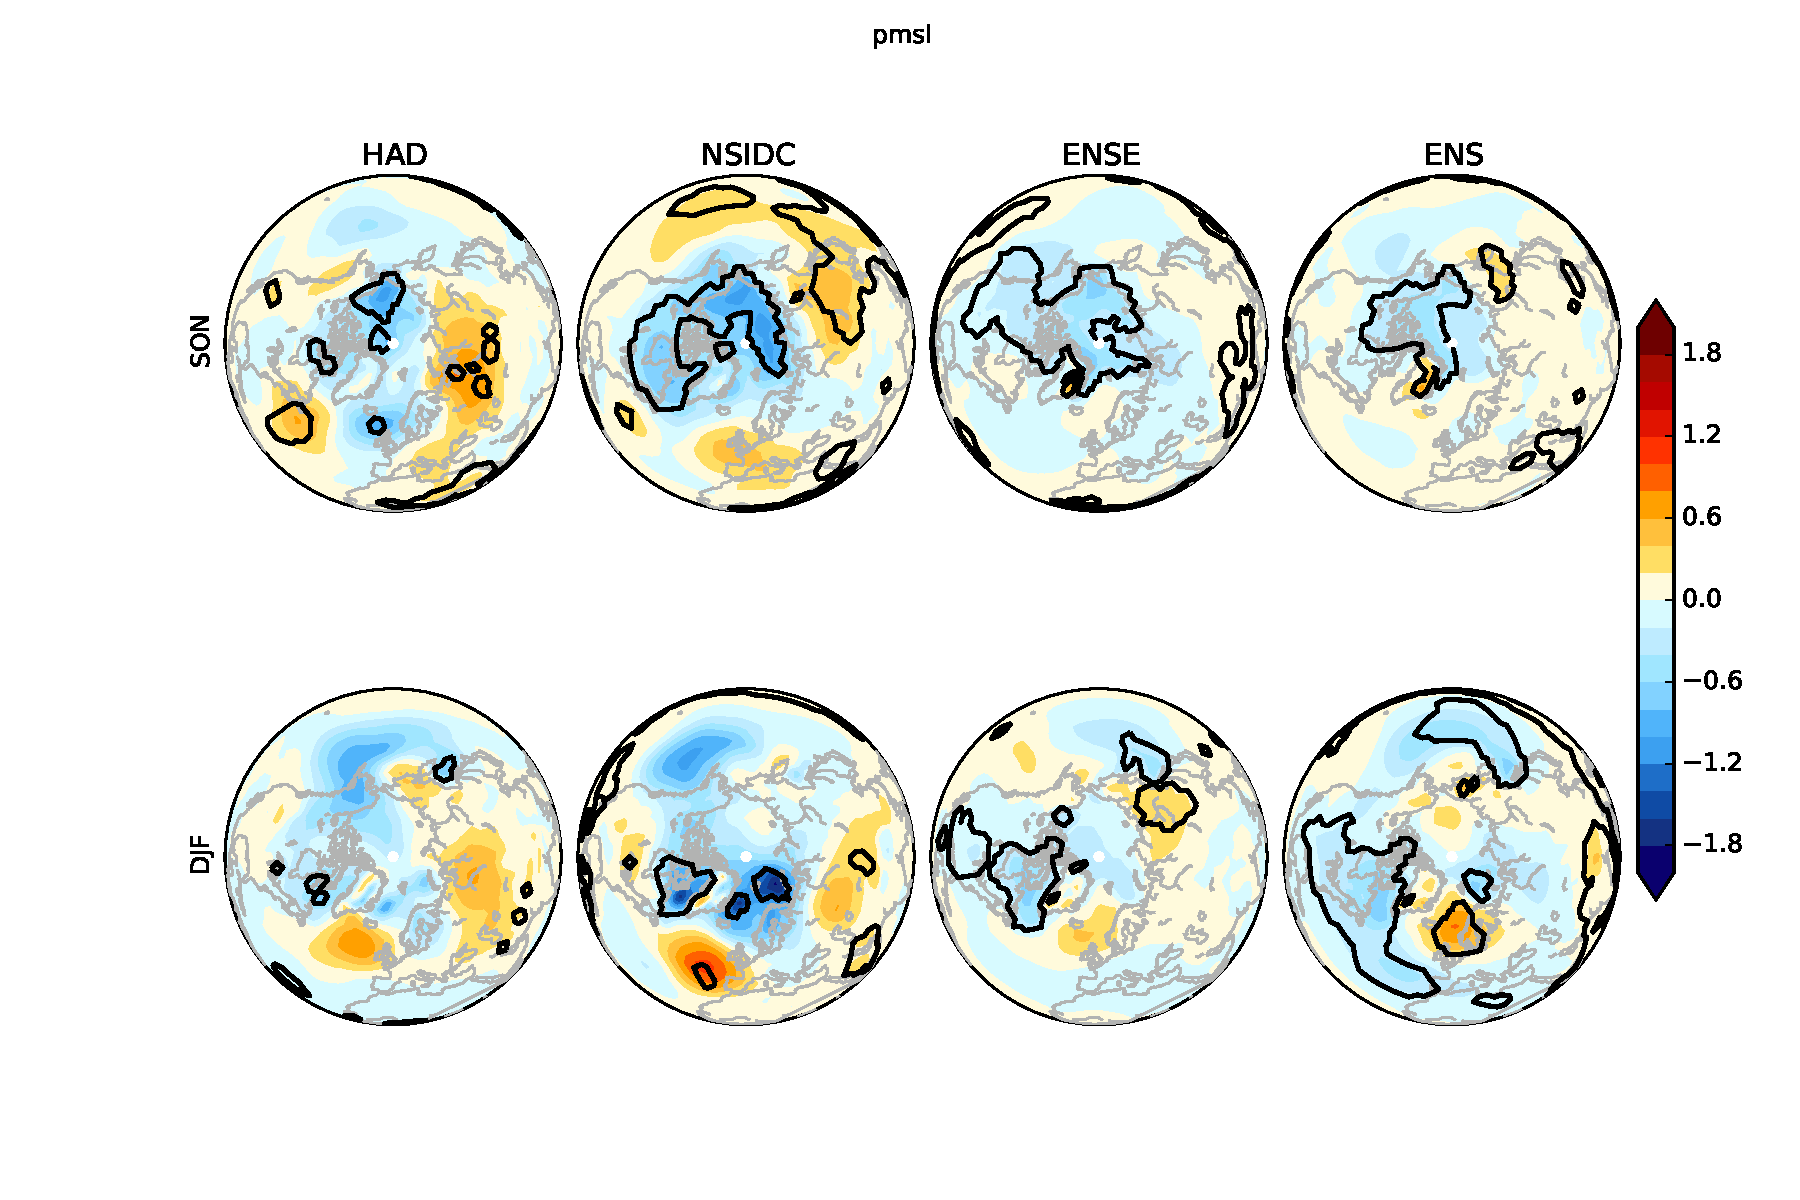
\includegraphics[width=35pc,angle=0]{pmsldiffsigcont_enssubplot_forpap3_seas_nh2.pdf} \\ %{SLPmaps.pdf}\\
  \caption{SLP maps.
}\label{fig:fig3b}
\end{figure*}

\begin{figure*}[t]
  \noindent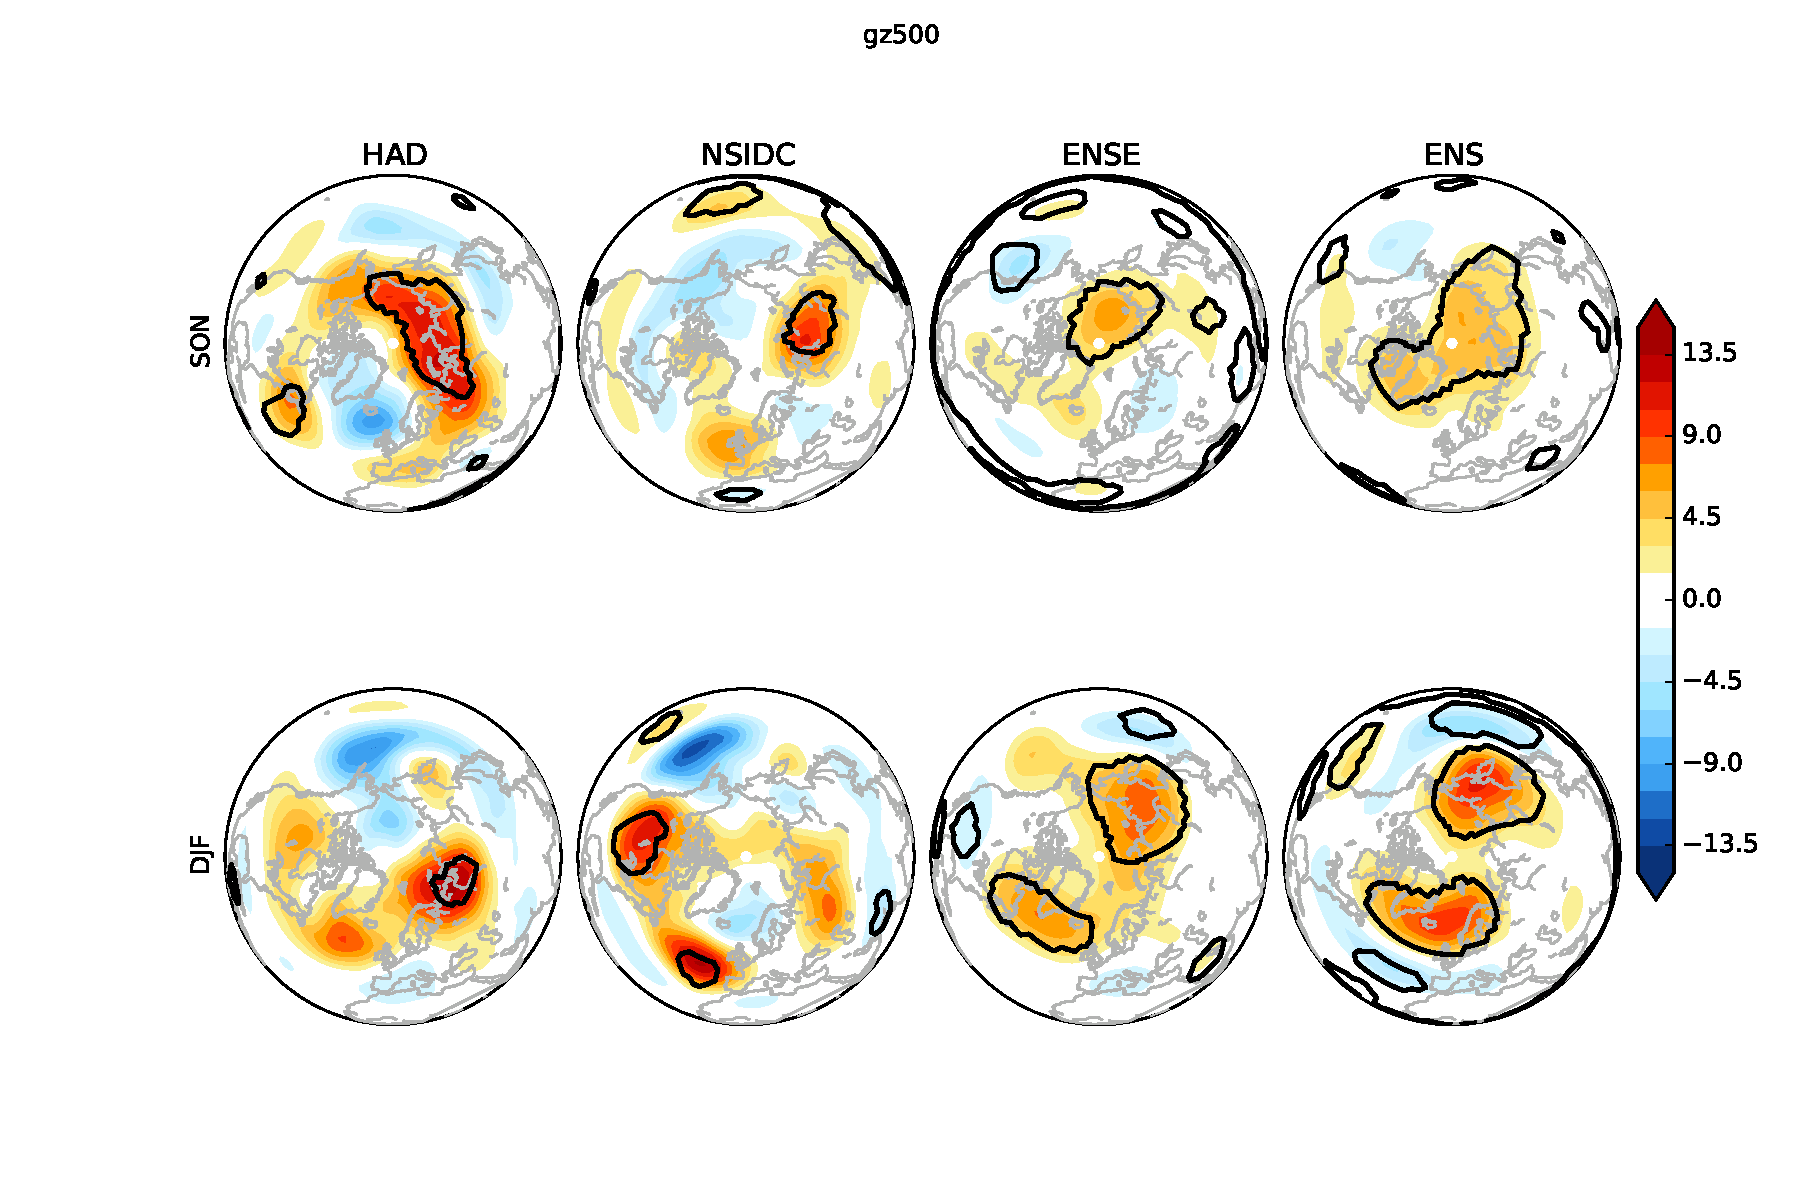
\includegraphics[width=35pc,angle=0]{gz500diffsigcont_enssubplot_forpap3_seas_nh2.pdf}\\ % {GZ500maps.pdf}\\
  \caption{Z500 maps.
}\label{fig:fig3c}
\end{figure*}

\begin{figure*}[t]
  \noindent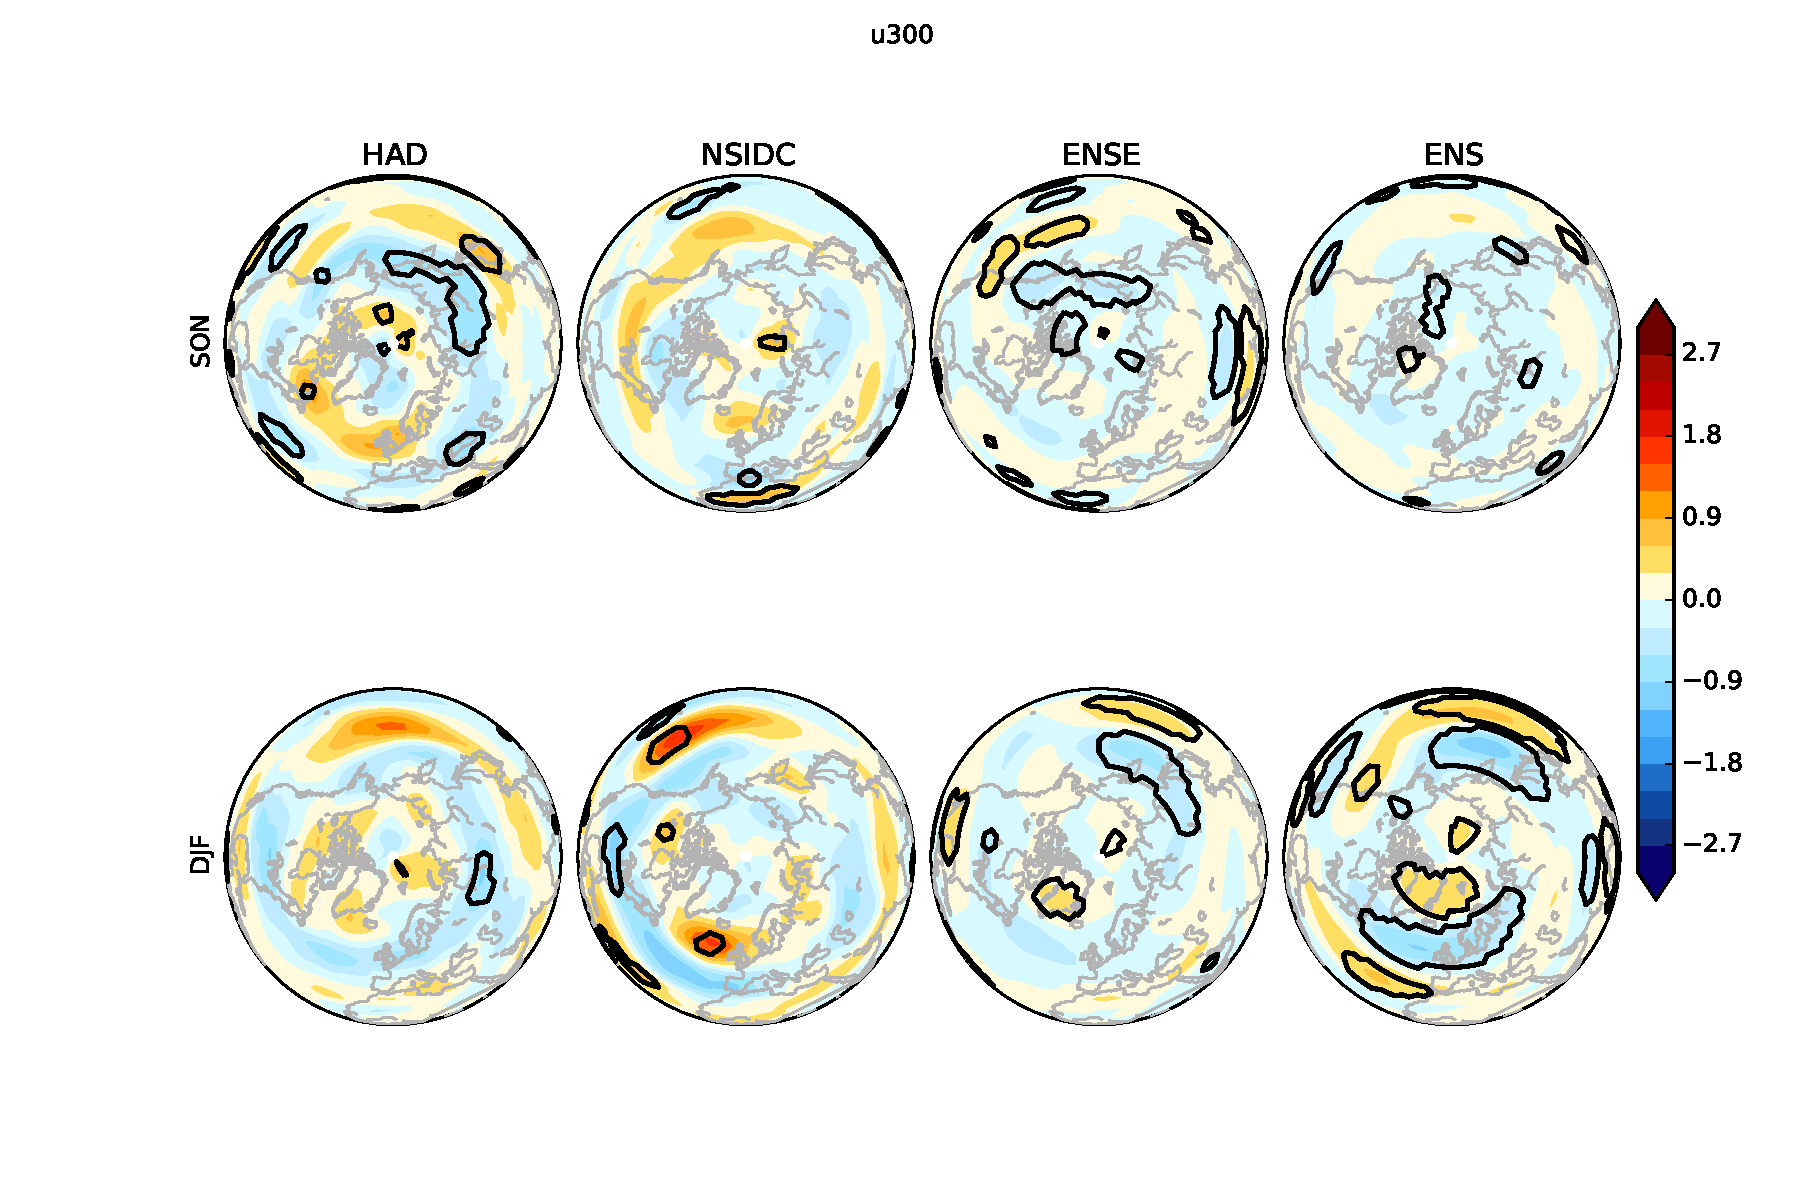
\includegraphics[width=35pc,angle=0]{u300diffsigcont_enssubplot_forpap3_seas_nh2.pdf}\\ % {GZ500maps.pdf}\\
  \caption{U300 maps.
}\label{fig:fig3d}
\end{figure*}

\begin{figure}[t]
  \noindent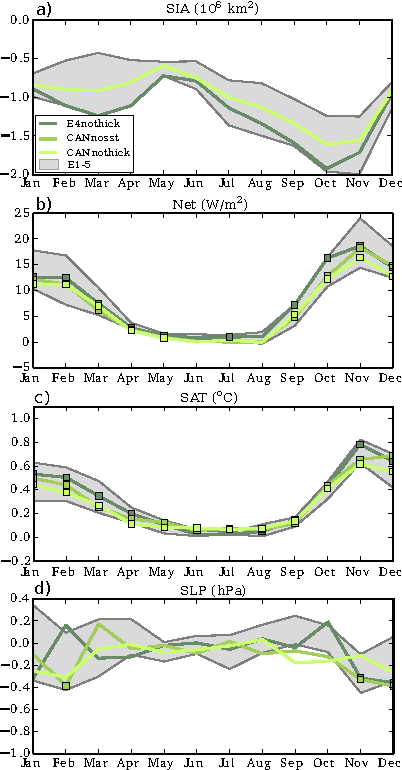
\includegraphics[width=15pc,angle=0]{seacyclessens.pdf}\\
  \caption{As Figure \ref{fig:fig2} but for the sensitivity runs TOT4nosit (dark green), ANT1nosst (medium green; exactly the same as ANT1nosit for sea ice area), and ANT1nosit (light green). 
}\label{fig:fig2b}
\end{figure} % Seasonal cycle of a.) Arctic sea ice area anomaly (10$^6$ km$^2$) for the sensitivity simulations E4nothick (dark green), CANnosst (medium green; exactly the same as CANnosit for sea ice area), and CANnosit (light green). Gray shading indicates the range of sea ice area anomalies in individual ensemble members as in Fig. \ref{fig:fig2}. b.) is as a) but for net surface flux anomaly averaged north of 40$^\circ$N where sea ice concentration $>$ 10\%, c.) is as a) but for surface air temperature anomaly averaged north of 70$^\circ$N, and d.) is as a) but for sea level pressure averaged north of 70$^\circ$N. Squares in b), c), and d) indicate a statistically significant change at the 95\% level using a two-sided student's T test. 

\begin{figure*}[t]
  \noindent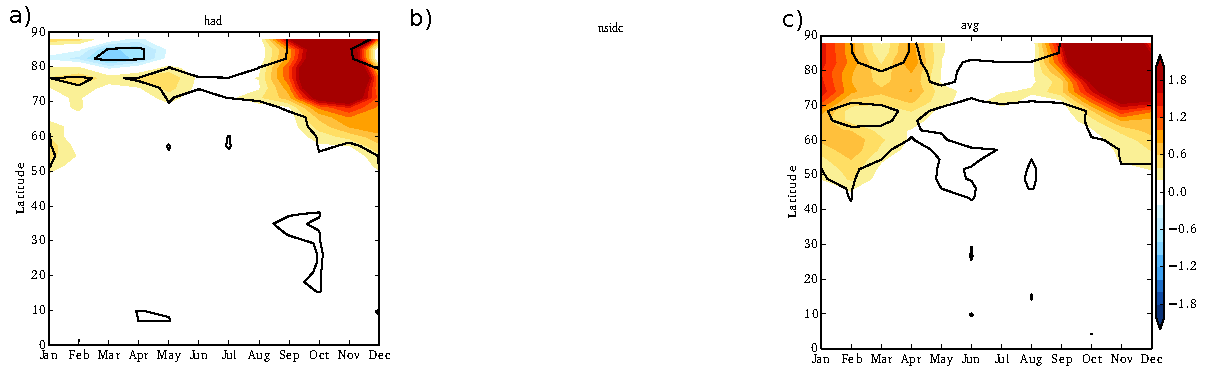
\includegraphics[width=39pc,angle=0]{SATwithlat.pdf}\\
  \caption{Zonal mean surface air temperature anomalies ($^\circ$C) by latitude and month for a.) HAD, b.) NSIDC, and c.) CAN. Black contours indicate statistically significant change at the 95\% level based on a two-sided student's T test. Gray contours show sea ice concentration anomalies for the respective simulations. Sea ice concentration anomalies have been multiplied by -1 for clarity.
}\label{fig:f1b}
\end{figure*}

\begin{figure}
  \noindent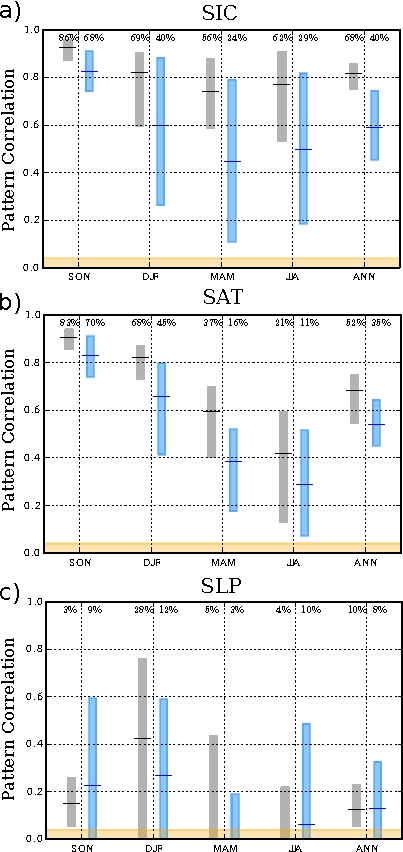
\includegraphics[width=15pc,angle=0]{pattcorrseas_cmpmeanBC.pdf}\\
  \caption{Pattern correlations (old)
}\label{fig:fig4}
\end{figure}

\clearpage

%\begin{figure}[t]
%  \noindent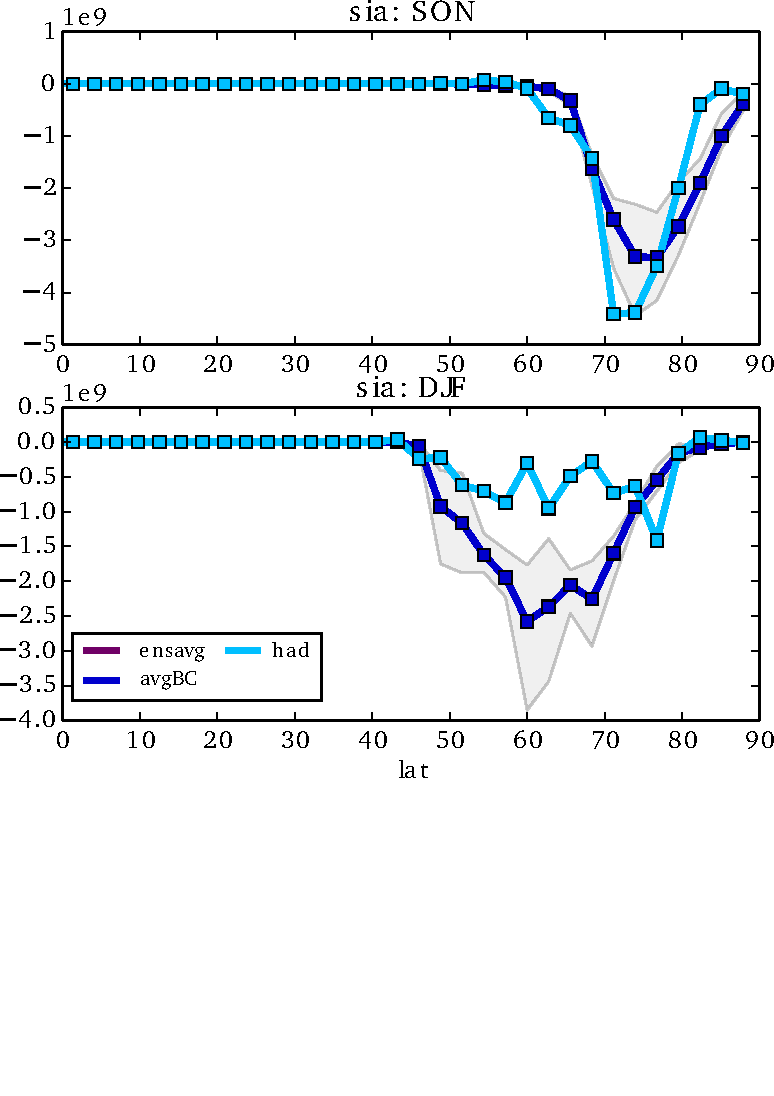
\includegraphics[width=19pc,angle=0]{SIAzonalmean.pdf}\\
%  \caption{Zonal mean sea ice area anomalies ($^\circ$C) with latitude for top) SON, bottom) DJF for the had simulations, avgBC simulations (blue), and the range of e1-5 simulations (gray shading). The mean of the ensemble is by definition the same as the avgBC simulations.
%}\label{f2}
%\end{figure}

%<<<<<<< HEAD
%\begin{figure*}[t]
%  \noindent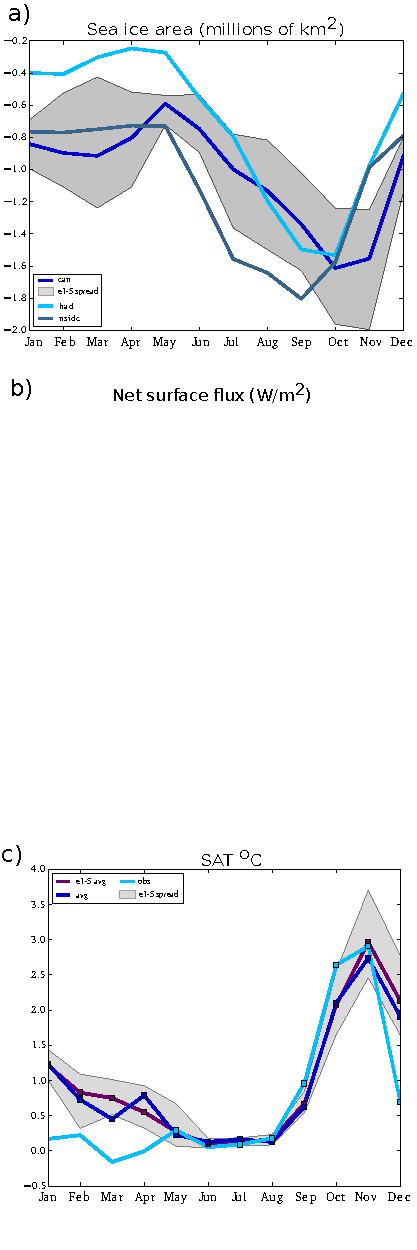
\includegraphics[width=39pc,angle=0]{seacycles.pdf}\\
%  \caption{@@Zonal mean surface air temperature anomalies ($^\circ$C) for a.) PTobs-CTLobs, b.) PTavg-CTLavg. c.) Seasonal cycle of area-averaged SAT North of 70$^\circ$N for all PT simulations and their respective CTL simulations. The gray shading indicates the range of e1-5 ensemble members. Note that here 'obs' indicates the simulations run with boundary conditions derived from observations (HadISST1.1).
%}\label{fig:fig2}
%\end{figure*}
%=======
%
%>>>>>>> FETCH_HEAD

%\begin{figure*}[t]
%  \noindent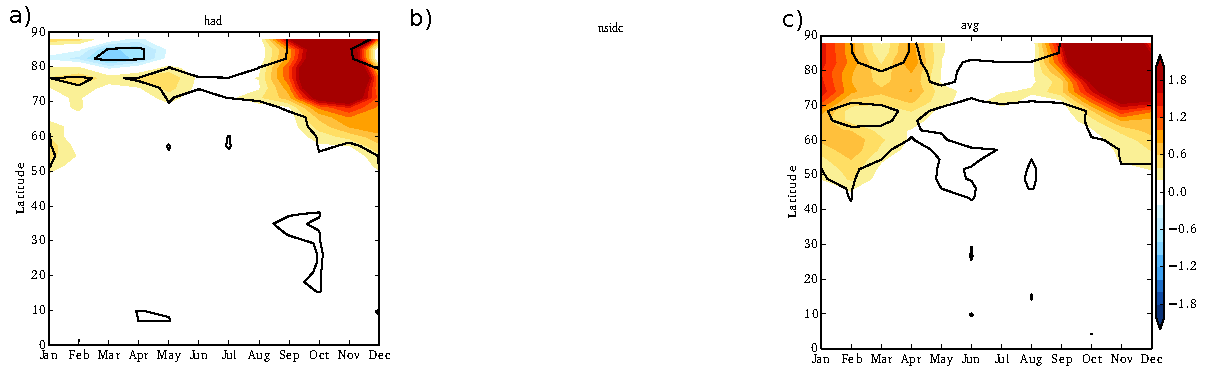
\includegraphics[width=39pc,angle=0]{SATwithlat.pdf}\\
%  \caption{Zonal mean surface air temperature anomalies ($^\circ$C) by latitude and month for a.) hadPT-hadCTL, b.) nsidcPT-nsidcCTL, and c.) canPT-canCTL. Black contours indicate statistically significant change at the 95\% level based on a two-sided student's T test.
%}\label{fig:fig3}
%\end{figure*}


%\begin{figure}[t]
%  \noindent\includegraphics[width=19pc,angle=0]{stdiff_ens_meanBC_allseassp_zonmean_nh2shade.pdf}\\
%  \caption{Zonal mean SAT anomalies ($^\circ$C) with latitude for the had simulations, avgBC simulations (blue), and the range of e1-5 simulations (gray shading). The mean of the ensemble is by definition the same as the avgBC simulations.
%}\label{f3}
%\end{figure}
%
%\begin{figure}[t]
%  \noindent\includegraphics[width=19pc,angle=0]{stdiff_ens_meanBC_r4ct_allseassp_zonmean_nh2.pdf}\\
%  \caption{Zonal mean SAT anomalies ($^\circ$C) with latitude for the had simulations, avgBC simulations (blue), and the range of e1-5 simulations (gray shading). The mean of the ensemble is by definition the same as the avgBC simulations.
%}\label{f4}
%\end{figure}


%%%%%%%%%%%%%%%%%%%%%%%%%%%%%%%%%%%%%%%%%%%%%%%%%%%%%%%%%%%%%%%%%%%%%
% ACKNOWLEDGMENTS
%%%%%%%%%%%%%%%%%%%%%%%%%%%%%%%%%%%%%%%%%%%%%%%%%%%%%%%%%%%%%%%%%%%%%
%
\acknowledgments
Start acknowledgments here.

%%%%%%%%%%%%%%%%%%%%%%%%%%%%%%%%%%%%%%%%%%%%%%%%%%%%%%%%%%%%%%%%%%%%%
% APPENDIXES
%%%%%%%%%%%%%%%%%%%%%%%%%%%%%%%%%%%%%%%%%%%%%%%%%%%%%%%%%%%%%%%%%%%%%
%
% Use \appendix if there is only one appendix.
%\appendix

% Use \appendix[A], \appendix}[B], if you have multiple appendixes.
%\appendix[A]

%% Appendix title is necessary! For appendix title:
%\appendixtitle{}

%%% Appendix section numbering (note, skip \section and begin with \subsection)
% \subsection{First primary heading}

% \subsubsection{First secondary heading}

% \paragraph{First tertiary heading}

%% Important!
%\appendcaption{<appendix letter and number>}{<caption>} 
%must be used for figures and tables in appendixes, e.g.,
%
%\begin{figure}
%\noindent\includegraphics[width=19pc,angle=0]{figure01.pdf}\\
%\appendcaption{A1}{Caption here.}
%\end{figure}

%%%%%%%%%%%%%%%%%%%%%%%%%%%%%%%%%%%%%%%%%%%%%%%%%%%%%%%%%%%%%%%%%%%%%
% REFERENCES
%%%%%%%%%%%%%%%%%%%%%%%%%%%%%%%%%%%%%%%%%%%%%%%%%%%%%%%%%%%%%%%%%%%%%
% Make your BibTeX bibliography by using these commands:
% \bibliographystyle{ametsoc2014}
% \bibliography{references}


%%%%%%%%%%%%%%%%%%%%%%%%%%%%%%%%%%%%%%%%%%%%%%%%%%%%%%%%%%%%%%%%%%%%%
% TABLES
%%%%%%%%%%%%%%%%%%%%%%%%%%%%%%%%%%%%%%%%%%%%%%%%%%%%%%%%%%%%%%%%%%%%%
%% Enter tables at the end of the document, before figures.
%%
%
%\begin{table}[t]
%\caption{This is a sample table caption and table layout.  Enter as many tables as
%  necessary at the end of your manuscript. Table from Lorenz (1963).}\label{t1}
%\begin{center}
%\begin{tabular}{ccccrrcrc}
%\hline\hline
%$N$ & $X$ & $Y$ & $Z$\\
%\hline
% 0000 & 0000 & 0010 & 0000 \\
% 0005 & 0004 & 0012 & 0000 \\
% 0010 & 0009 & 0020 & 0000 \\
% 0015 & 0016 & 0036 & 0002 \\
% 0020 & 0030 & 0066 & 0007 \\
% 0025 & 0054 & 0115 & 0024 \\
%\hline
%\end{tabular}
%\end{center}
%\end{table}

%%%%%%%%%%%%%%%%%%%%%%%%%%%%%%%%%%%%%%%%%%%%%%%%%%%%%%%%%%%%%%%%%%%%%
% FIGURES
%%%%%%%%%%%%%%%%%%%%%%%%%%%%%%%%%%%%%%%%%%%%%%%%%%%%%%%%%%%%%%%%%%%%%
%% Enter figures at the end of the document, after tables.
%%
%
%\begin{figure}[t]
%  \noindent\includegraphics[width=19pc,angle=0]{figure01.pdf}\\
%  \caption{Enter the caption for your figure here.  Repeat as
%  necessary for each of your figures. Figure from \protect\cite{Knutti2008}.}\label{f1}
%\end{figure}

\end{document}